\documentclass[11pt,a4paper,english,greek,twoside]{auth-thesis}
\usepackage{epsfig}
%\usepackage[english,greek]{babel}
%\usepackage[T1]{fontenc}
%\usepackage[iso-8859-7]{inputenc}
%\usepackage{graphicx}
%\DeclareGraphicsRule{.tif}{bmp}{}{}
\usepackage[explicit]{titlesec}
\usepackage{indentfirst}
\usepackage{verbatim}
\usepackage{amsmath}
\usepackage{subcaption}
\usepackage{amsthm}
\usepackage{amssymb}
\usepackage{epstopdf}
\usepackage{latexsym}
\usepackage{index}
\usepackage{datetime}
\usepackage{textcomp}
\usepackage{graphicx}
\usepackage{url}
\usepackage{array}
\usepackage{algorithm}
\usepackage{algorithmic}
\usepackage{babel}
\usepackage{afterpage}
\usepackage{caption}
%\usepackage{makeidx}
%\bibliographystyle{alpha}
\bibliographystyle{abbrv}

\newindex{default}{idx}{ind}{Ευρετήριο όρων}
\newindex{en}{edx}{end}{Ευρετήριο αγγλικών όρων}
%\makeindex


% Page definitions
%\setlength{\textheight}{23cm} \setlength{\textwidth}{15.5cm}
%\setlength{\oddsidemargin}{0.2cm}
%\setlength{\evensidemargin}{0.2cm} \setlength{\topmargin}{-1.2cm}
%\setlength{\headsep}{1.5cm}

% 1.5 spacing
\renewcommand{\baselinestretch}{1.2}

\newcommand\blankpage{%
    \null
    \thispagestyle{empty}%
    \addtocounter{page}{-1}%
    \newpage}
% latin text (and greek text)
%\newcommand{\prg}[1]{\textlatin{\texttt{#1}}}
\newcommand{\tl}[1]{\textlatin{#1}}
\newcommand{\tg}[1]{\textgreek{#1}}

% typeset short english phrases
\newcommand{\en}[1]{\foreignlanguage{english}{#1}}

% typeset source code
\newcommand{\src}[1]{{\tt\en{#1}}}



% typeset a backslash
\newcommand{\bkslash}{\en{\symbol{92}}}

%typeset infx(a) supx(a) etc
%\newcommand{\infx}[1]{inf_x({#1})}
%\newcommand{\infy}[1]{inf_y({#1})}
%\newcommand{\supx}[1]{sup_x({#1})}
%\newcommand{\supy}[1]{sup_y({#1})}
%\newcommand{\dlt}{\delta}
%\newcommand{\most}{${\cal M}ost$}
%\newcommand{\br}{${\cal B}r$}
\newcommand*\Hide{%
\titleformat{\chapter}[display]
  {}{}{0pt}{\Huge}
\titleformat{\part}
  {}{}{0pt}{}
}
\newtheorem{definition}{Ορισμός}
\newtheorem{proposition}{Πρόταση}
\newtheorem{theorem}{Θεώρημα}
\newtheorem{corollary}{Συμπέρασμα}
\newtheorem{lemma}{Λήμμα}
\newtheorem{example}{Παράδειγμα}
\newtheorem{remark}{Σημείωση}
\newtheorem{notation}{Συμβολισμός}
\newtheorem{law}{Νόμος}
\renewcommand{\thedefinition}{\arabic{chapter}.\arabic{definition}}
\renewcommand{\theproposition}{\arabic{chapter}.\arabic{proposition}}
\renewcommand{\thetheorem}{\arabic{chapter}.\arabic{theorem}}
\renewcommand{\thecorollary}{\arabic{chapter}.\arabic{corollary}}
\renewcommand{\thelemma}{\arabic{chapter}.\arabic{lemma}}
\renewcommand{\theexample}{\arabic{chapter}.\arabic{example}}
\newcommand{\set}[1]{\left\{#1\right\}}
\newcommand{\To}{\Longrightarrow}
\newcommand{\xml}{\en{XML}}


\selectlanguage{greek}
\hyphenation{τμή-μα Επο-μέ-νως}

\title{Ηλεκτρομαγνητική προσομοίωση ενός \en{Electron Beam Scanner} για μικρές δέσμες}
\author{Ορφέας Αντωνίου}
\supervisor{Νικόλαος Κανταρτζής}
\TRnumber{ΕΣΒΓΔ-ΔΙΠΛ-2015-03} %TODO update
\epitropiF{Νικόλαος Κανταρτζής} %TODO update
\epitropiS{Νικόλαος Κανταρτζής} %TODO update


\begin{document}

\selectlanguage{greek}
\maketitle

\frontmatter
\pagenumbering{roman}
\mainmatter
\begin{acknowledgements}
Θα ήθελα αρχικά να ευχαριστήσω τον καθηγητή κ. Ανδρέα Συμεωνίδη για την εμπιστοσύνη και την καθοδήγηση 
και τον κ. Κυριάκο Χατζηδημητρίου για την καθοδήγηση και τη συνεργασία στα πλαίσια αυτής της διπλωματικής εργασίας. Επίσης θέλω να ευχαριστήσω την οικογένειά μου για την αδιάληπτη στήριξη όλα αυτά τα χρόνια.
\end{acknowledgements}

\begin{abstract}
Η περίληψη θα συμπληρωθεί αργότερα. Αυτή είναι μια περίληψη άλλης εργασίας:

Ένα σύστημα ομότιμων κόμβων αποτελείται από ένα σύνολο αυτόνομων
υπολογιστικών κόμβων στο Διαδίκτυο, οι οποίοι συνεργάζονται με
σκοπό την ανταλλαγή δεδομένων. Στα συστήματα ομότιμων κόμβων που
χρησιμοποιούνται ευρέως σήμερα, η αναζήτηση πληροφορίας γίνεται με
χρήση λέξεων κλειδιών. Η ανάγκη για πιο εκφραστικές λειτουργίες,
σε συνδυασμό με την ανάπτυξη του Σημασιολογικού Ιστού, οδήγησε στα
συστήματα ομότιμων κόμβων βασισμένα σε σχήματα. Στα συστήματα αυτά
κάθε κόμβος χρησιμοποιεί ένα σχήμα με βάση το οποίο οργανώνει τα
τοπικά διαθέσιμα δεδομένα. Για να είναι δυνατή η αναζήτηση
δεδομένων στα συστήματα αυτά υπάρχουν δύο τρόποι. Ο πρώτος είναι
όλοι οι κόμβοι να χρησιμοποιούν το ίδιο σχήμα κάτι το οποίο δεν
είναι ευέλικτο. Ο δεύτερος τρόπος δίνει την αυτονομία σε κάθε
κόμβο να επιλέγει όποιο σχήμα θέλει και απαιτεί την ύπαρξη κανόνων
αντιστοίχισης μεταξύ των σχημάτων για να μπορούν να αποτιμώνται οι
ερωτήσεις. Αυτός ο τρόπος προσφέρει ευελιξία όμως δεν υποστηρίζει
την αυτόματη δημιουργία και τη δυναμική ανανέωση των κανόνων, που
είναι απαραίτητες για ένα σύστημα ομότιμων κόμβων.

Στόχος της διπλωματικής εργασίας είναι η ανάπτυξη ενός συστήματος
ομότιμων κόμβων βασισμένο σε σχήματα το οποίο (α) θα επιτρέπει μια
σχετική ευελιξία στην χρήση των σχημάτων και (β) θα δίνει την
δυνατότητα μετασχηματισμού ερωτήσεων χωρίς την ανάγκη διατύπωσης
κανόνων αντιστοίχισης μεταξύ σχημάτων, xρησιμοποιώντας κόμβους με
σχήματα \tl{RDF} που αποτελούν υποσύνολα-όψεις ενός βασικού
σχήματος (καθολικό σχήμα).


   \begin{keywords}
   Σύστημα ομότιμων κόμβων, Σύστημα ομότιμων κόμβων βασισμένο σε
   σχήματα, Σημασιολογικός Ιστός, \tl{RDF/S}, \tl{RQL}, \tl{Jxta}
   \end{keywords}
\end{abstract}



\begin{abstracteng}
\tl{This is a placeholder for the abstract of my thesis. The actual abstract is going to be written after I finish all chapters.

The Compact LInear Collider (CLIC) will use a novel acceleration scheme in which energy extracted from a very intense beam of relatively low-energy electrons (the Drive Beam) is used to accelerate a lower intensity Main Beam to very high energy. The high intensity of the Drive Beam, with pulses of more than $10^{15}$ electrons, poses a challenge for conventional profile measurements such as wire scanners. Thus, new non-invasive profile measurements are being investigated.}

\tl{One candidate is the Electron Beam Scanner. A probe beam of low-energy electrons crosses the accelerator beam perpendicularly. The probe beam is deflected by the space-charge fields of the accelerator beam. By scanning the probe beam and measuring its deflection with respect to its initial position, the transverse profile of the accelerator beam can be reconstructed.}

\tl{Analytical expressions for the deflection exist in the case of long bunches, where the charge distribution can be considered constant during the measurement. In this paper we consider the performance of an electron beam scanner in an accelerator where the bunch length is much smaller than the probe-beam scanning time. In particular, the case in which the bunch length is shorter than the time taken for a particle of the probe beam to cross the main beam is difficult to model analytically. We have developed a simulation framework allowing this situation to be modelled.}

   \begin{keywordseng}
    \tl{Fill in }
    %TODO fill in keywords
   \end{keywordseng}

\end{abstracteng}
 % abstract and acknowledgements
%TODO write abstract
\tableofcontents
\listoffigures
\listoftables
\chapter{Εισαγωγή}
%Εισαγωγικά, γιατί διάλεξα CST

\begin{enumerate}
\item \en{about CERN}
\item \en{about CLIC}
\end{enumerate}

Το \en{CERN} μπλα μπλα μπλα.

Το \en{CLIC} μπλα μπλα μπλα.

Μέχρι στιγμής οι τρόποι ανίχνευσης μπλα μπλα μπλα.
Μη επεμβατικοί τρόποι πρέπει να πάρουν θέση. Ένας είναι το \en{Electron Beam Scanner}. Παρόλα αυτά μικρή δέσμη στο \en{CLIC}. 

\section{Αντικείμενο της διπλωματικής}
Σκοπός είναι να δούμε αν μπορούμε να χρησιμοποιήσουμε τον \en{Electron Beam Scanner} για να πάρουμε την εικόνα της δέσμη του \en{CLIC}.

\section{Οργάνωση του τόμου}
Η εργασία αυτή είναι οργανωμένη σε πέντε κεφάλαια: Στο Κεφάλαιο 2
δίνεται το θεωρητικό υπόβαθρο των βασικών τεχνολογιών που
σχετίζονται με τη διπλωματική αυτή. Αρχικά περιγράφονται ..., στη συνέχεια το ... και τέλος ... . 
Στο Κεφάλαιο 3 αρχικά παρουσιάζεται ανάλυση και η σχεδίαση του συστήματος ... .. Τέλος στο Κεφάλαιο 5 δίνονται τα συμπεράσματα, η συνεισφορά αυτής της
διπλωματικής εργασίας, καθώς και μελλοντικές επεκτάσεις.

\chapter{\selectlanguage{greek}Θεωρητικό υπόβαθρο}
\begin{itemize}
\item περιγραφή πειράματος και
\item Για να καταλάβει ο κόσμος τι σημαίνει
\item Γιατί είναι χρήσιμο
\item Φωτογραφίες
\item Τι χρειάζεται να ξέρω
\item Το πείραμα
\end{itemize}

Στο κεφάλαιο αυτό παρουσιάζονται αναλυτικά οι 

\section{\selectlanguage{greek}Το \en{CERN}}

To \en{CERN}, διατηρώντας το ακρωνύμιο της αρχικής Γαλλικής ονομασίας του \en{Conseil Européen pour la Recherche Nucléaire}, είναι το μεγαλύτερο σε έκταση πειραματικό κέντρο πυρηνικών ερευνών και ειδικότερα επί της σωματιδιακής φυσικής στον κόσμο. 
Βρίσκεται δυτικά της Γενεύης, στα σύνορα Ελβετίας και Γαλλίας. 
Ιδρύθηκε το 1954 από 12 ευρωπαϊκές χώρες και σήμερα αριθμεί 20 κράτη-μέλη, μεταξύ των οποίων και η Ελλάδα, η οποία είναι και ιδρυτικό μέλος.

\begin{figure}[h]

\includegraphics[scale=0.7]{images/LogoBadge-01.png}
\centering
\caption{Το λογότυπο του \en{CERN}}
\label{CERNlogo}
\end{figure}

Η βασική λειτουργία του \en{CERN} είναι η παροχή επιταχυντών σωματιδίων και άλλων υποδομών απαραίτητων για την έρευνα στον τομέα της φυσικής υψηλών ενεργειών και ως αποτέλεσμα έχουν πραγματοποιηθεί πολυάριθμα πειράματα στο \en{CERN} μέσω διεθνών συνεργασιών.

Επίσης, το \en{CERN} αποτελεί τη γενέτειρα του Παγκόσμιου Ιστού (\en{World Wide Web}).
Στην κύρια τοποθεσία του στο \en{Meyrin} βρίσκεται μεγάλη εγκατάσταση ηλεκτρονικών υπολογιστών με ισχυρές υποδομές επεξεργασίας δεδομένων, κυρίως για την ανάλυση των πειραματικών δεδομένων. 
Λόγω της ανάγκης να καταστούν αυτές διαθέσιμες σε εξωτερικούς ερευνητές, υπήρξε ιστορικά ένας σημαντικός κόμβος δικτύου ευρείας περιοχής (\en{Wide Area Network}).

Αρκετά σημαντικά επιτεύγματα στο πεδίο της φυσικής των σωματιδίων έγιναν μέσω πειραμάτων στο \en{CERN}. Αυτά περιλαμβάνουν:
\begin{itemize}
\item 1973: Ανακάλυψη των ουδέτερων ρευμάτων στο θάλαμο φυσαλίδων \en{Gargamelle}.
\item 1983: Ανακάλυψη των μποζονίων $W$ και $Z$ στα πειράματα \en{UA1} και \en{UA2}.
\item 1995: Πρώτη δημιουργία ατόμων αντιυδρογόνου στο πείραμα \en{PS210}.
\item 1999: Ανακάλυψη της άμεσης παραβίασης \en{CP} στο πείραμα \en{NA48}.
\item 2010: Απομόνωση 38 ατόμων αντιυδρογόνου.
\item 2011: Διατήρηση αντιυδρογόνου για πάνω από 15 λεπτά.
\item 2012: Ένα μποζόνιο με μάζα περίπου \SI[per-mode = symbol]{125}{\GeV \per  \clight \squared} συνάδει με τον πολυπόθητο μποζόνιο \en{Higgs}.
\end{itemize}


\section{\selectlanguage{greek}Ο επιταχυντής \en{CLIC}}

Ο \en{CLIC -- Compact Linear Collider} -- αποτελεί μια μελέτη για ένα μελλοντικό επιταχυντή που θα φτάσει σε πρωτοφανή επίπεδα ενέργειας ηλεκτρόνια και αντισωμάτιά τους, ποζιτρόνια. 
Όταν θα έρχονται σε επαφή μέσω σύγκρουσης, θα καταστρέφουν το ένα το άλλο, απελευθερώνοντας όλη τους την ενέργεια για την παραγωγή νέων σωματιδίων.

Τα ηλεκτρόνια και τα ποζιτρόνια είναι θεμελιώδη σωματίδια και οι συγκρούσεις τους μπορούν να προσφέρουν εξαιρετικά λεπτομερείς πληροφορίες σχετικά με τους νόμους της φύσης. 
Έτσι ο \en{CLIC} θα προσφέρει σημαντικές θεμελιώδεις γνώσεις φυσικής, πέρα από αυτές που είναι διαθέσιμες από το Μεγάλο Επιταχυντή Αδρονίων (\en{Large Hadron Collider -- LHC}) ή από ένα γραμμικό επιταχυντή ηλεκτρονίων/ποζιτρονίων χαμηλότερης ενέργειας, λόγω του μοναδικού συνδυασμού πειραματικής ακρίβειας και υψηλής ενέργειας.

Σε αυτές τις υψηλές ενέργειες, τα ηλεκτρόνια και ποζιτρόνια θα έχαναν ένα τεράστιο μέρος της ενέργειάς τους επιταχυνόμενα σε έναν κυκλικό επιταχυντή σαν τον \en{LHC}. 
Έτσι, τα σωματίδια πρέπει να επιταχυνθούν σε δύο γραμμικούς επιταχυντές που αντικρίζουν ο ένας τον άλλο, έτσι ώστε οι δέσμες να συγκρούονται στον κεντρικό ανιχνευτή. 
Αυτό συνεπάγεται ότι τα σωματίδια πρέπει να αποκτήσουν την ενέργειά τους από ένα και μόνο πέρασμα τους μέσα από τις κοιλότητες επιτάχυνσης.

\begin{figure}[h]
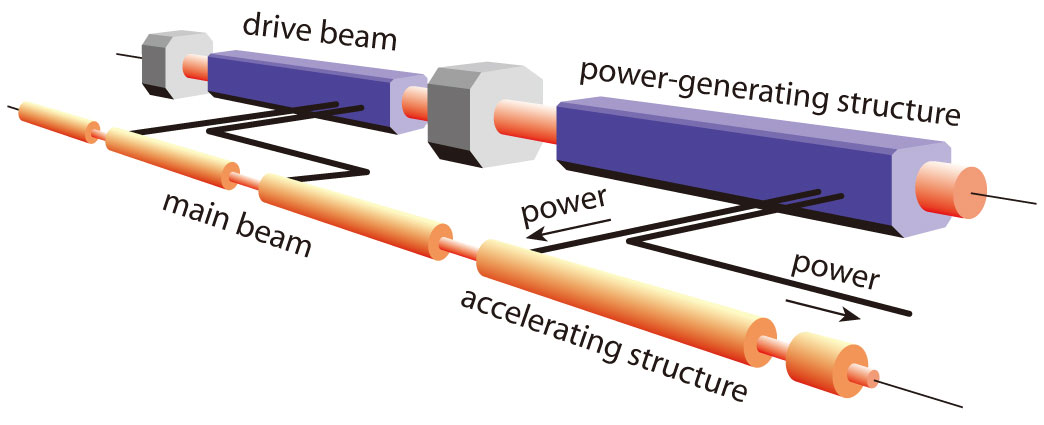
\includegraphics[width=0.5\textwidth]{images/CLIC-twobeam.jpg}
\centering
\caption{Το σύστημα δύο δεσμών του \en{CLIC}}
\label{CLICtwobeamscheme}
\end{figure}

Ο \en{CLIC} έχει σχεδιαστεί για να κατασκευαστεί σε στάδια αυξανόμενης ενέργειας για σύγκρουση: ξεκινώντας από \SI{360}{\GeV}, περίπου \SI{1.4}{\TeV}, και μέχρι την τελική ενέργεια των \SI{3}{\TeV}. 
Προκειμένου να επιτευχθεί αυτή η ενέργεια με ένα ρεαλιστικό και οικονομικά αποδοτικό τρόπο, η αύξηση της επιτάχυνσης πρέπει να είναι πολύ υψηλή.
Ο \en{CLIC} αποσκοπεί σε επιτάχυνση των \SI[per-mode = symbol]{100}{\mega \volt \per \metre}, 20 φορές υψηλότερη από αυτή του \en{LHC}.

Αυτή η δέσμη-οδηγός (drive beam) επιβραδύνεται σε ειδικές Διατάξεις Εξαγωγής και Mεταφοράς Ισχύος -- \en{Power Extraction and Transfer Structures (PETS)}, και η παραγόμενη \en{RF} ισχύς μεταφέρεται στην κύρια δέσμη. 
Αυτό οδηγεί σε μια πολύ απλή διάταξη σήραγγα χωρίς ενεργά \en{RF} μέρη (δηλ. \en{klystrons}).

\begin{figure}[h]
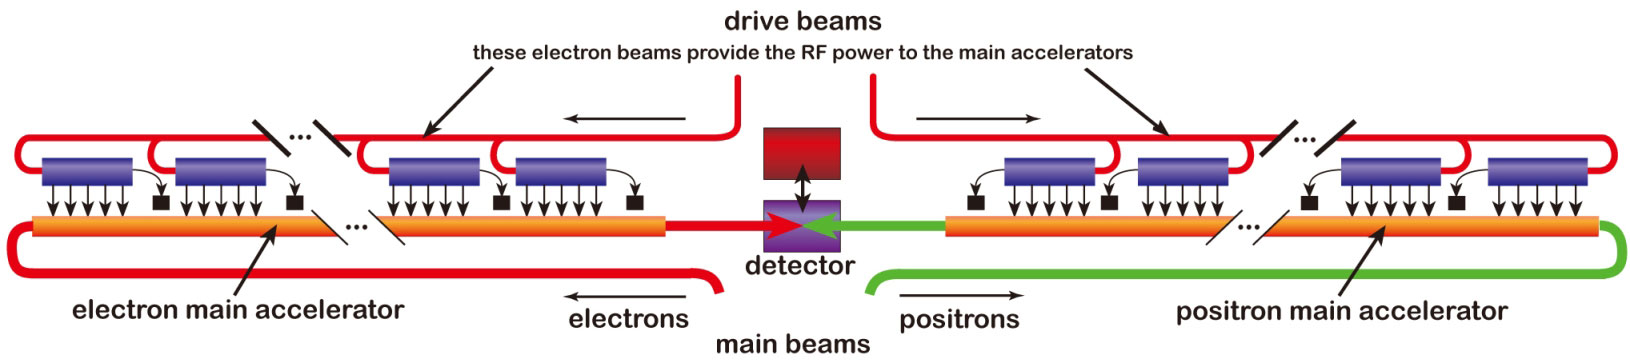
\includegraphics[width=\textwidth]{images/CLIC-layout.jpg}
\centering
\caption{Το σχεδιάγραμμα του \en{CLIC}}
\label{CLIClayout}
\end{figure}

Ο \en{CLIC} είναι μία από τις επιλογές για έναν μελλοντική επιταχυντή κατασκευασμένο στο \en{CERN}, το οποίο θα αποφασιστεί ανάλογα με τα μελλοντικά αποτελέσματα του \en{LHC}.

\section{\selectlanguage{greek}Το \en{Electron beam scanner}}


\chapter{Σχετική βιβλιογραφία}

Στο κεφάλαιο αυτό παρουσιάζουμε σχετικές προσεγγίσεις και υλοποιήσεις στο πρόβλημα του αυτόματου προγραμματισμού και της παραγωγής κώδικα.
Επειδή είναι πρακτικά αναρίθμητες, θα επικεντρωθούμε σε αυτές που είναι σχετικές με τα αναδραστικά νευρωνικά δίκτυα και σε κάποιες που παρουσιάζουν ιδιαίτερο ενδιαφέρον.

\section{\en{Generating Sequence with Recurrent Neural Networks}}
Στην εργασία των \en{Graves et al.} παρουσιάζεται πως απλές δομές αναδραστικών νευρωνικών δικτύων με στοιχεία μνήμης \en{LSTM} μπορούν να χρησιμοποιηθούν για να παράξουν σύνθετες ακολουθίες, απλά προβλέποντας ένα στοιχείο της ακολουθίας τη φορά. 
Θεωρώντας τις προβλέψεις στοχαστικές, καινούριες ακολουθίες μπορούν να προκύψουν από ένα εκπαιδευμένο δίκτυο, δειγματοληπτώντας επαναληπτικά από την έξοδο του δικτύου και ύστερα ξανά-δίνοντας ως είσοδο στο δικτύου την δειγματοληπτημένη πρόβλεψη.
Με μία διαφορετική διατύπωση, αφήνουμε το δίκτυο να αντιμετωπίσει τις επινοήσεις του ως αληθινές, περίπου σαν έναν άνθρωπο ο οποίος ονειρεύεται. 
Αν και το σύστημα είναι ντετερμινιστικό, η στοχαστικότητα που εισάγεται δειγματοληπτώντας δημιουργεί μία κατανομή σε σχέση με τις ακολουθίες.
Αυτή η κατανομή είναι δεσμευμένη, αφού η εσωτερική αναπαράσταση του δικτύου, άρα και κατανομή προβλέψεων του, εξαρτάται από τις προηγούμενες εισόδους.

Η προσέγγιση αυτή επιδεικνύεται για κείμενο (όπου οι τιμές είναι διακριτές) και για <<\en{online}>>  χειρόγραφο κείμενο (όπου οι τιμές είναι πραγματικές).
Με τον όρο <<\en{online}>> εννοούμε ότι η γραφή αποτυπώνεται ως ακολουθία διανυσμάτων θέσης ενός μολυβιού -- σε αντίθεση με το <<\en{offline}>> στο οποίο έχουμε διαθέσιμη ολόκληρη την εικόνα του χειρόγραφου.
Το σύστημα που χρησιμοποιείται είναι μια συστάδα που αποτελείται από 7 επίπεδα αναδραστικών νευρωνικών δικτύων με 700 στοιχεία μνήμης \en{LSTM}.
Για την παραγωγή ακολουθιών κειμένου χρησιμοποιούνται τρία διαφορετικά σετ δεδομένων. Το Penn Treebank και το Wikipedia Hutter Prize για το γραπτό κείμενο και το <<\en{IAM online handwriting database}>>.
Το μοντέλο καταφέρνει να παράξει ακολουθίες τόσο ρεαλιστικές ώστε να είναι συχνά δύσκολο να τις ξεχωρίσει κανείς από πραγματικές, τουλάχιστον σε πρώτη όψη.
Στα αποτελέσματα είναι ορατή μια μεγάλης εμβέλειας δομή και συνοχή.

\begin{figure}[tph]
	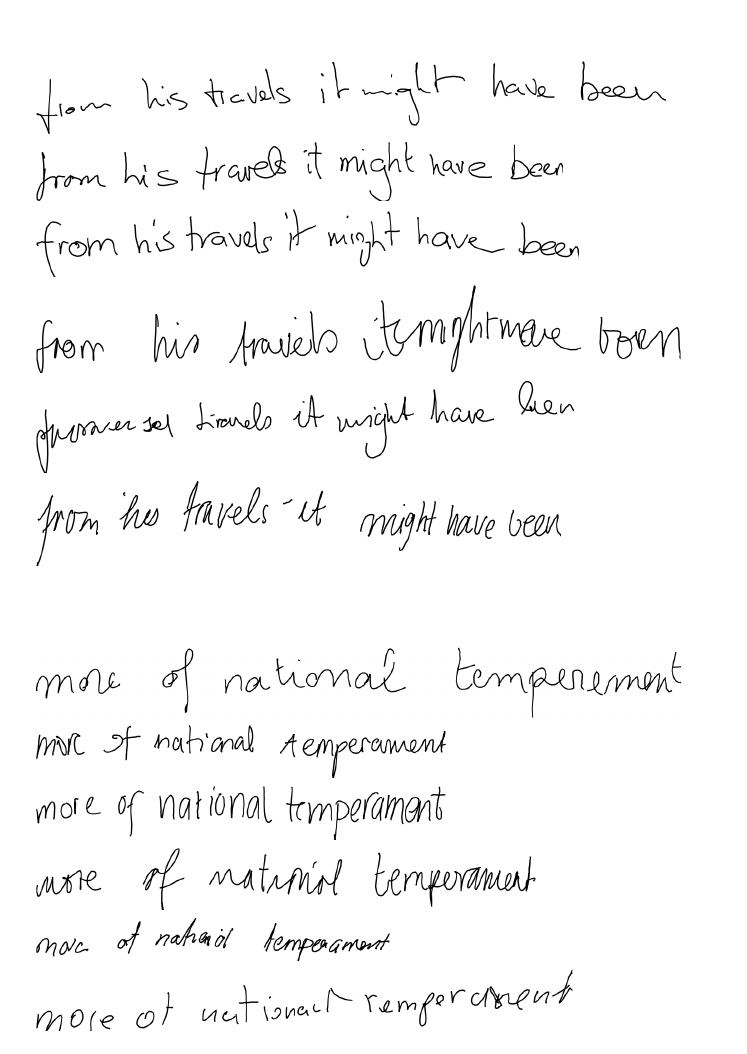
\includegraphics[width=\textwidth, keepaspectratio]{images/handwriting.png}
	\centering 
	\caption{Ένα τυπικό δομικό διάγραμμα επιτηρούμενης εκμάθησης.}
	\label{fig:training}
\end{figure}

Επιπρόσθετα, βασισμένοι στην προηγούμενη δομή, οι \en{Graves et al.} σχεδιάζουν ένα σύστημα παραγωγής χειρόγραφου κειμένου το οποίο μπορεί να γράψει αυτό που του ζητάμε.
Αυτό γίνεται με την προσθήκη ενός διανύσματος της πρότασης που θέλουμε να γράψουμε, το οποίο δίνεται στο σύστημα πρόβλεψης την ώρα της παραγωγής, αφού προφανώς εκπαιδευτεί σε σχετικά προβλήματα.
Η απόφαση για το πότε και πως θα γραφεί κάθε χαρακτήρας αφήνεται στο νευρωνικό δίκτυο και τα αποτελέσματα είναι αρκετά ικανοποιητικά ώστε να είναι και πάλι δύσκολο να διακριθεί αν τα <<χειρόγραφα>> ανήκουν σε κάποιον άνθρωπο ή στο σύστημα.

\section{\en{Inferring Algorithmic Patterns with Stack-Augmented Recurrent Nets}}

Οι \en{Joulin et al.} στην έρευνα τους εξετάζουν τα όρια των \en{"state of the art" Deep Learning} προσεγγίσεων.
Πιο συγκεκριμένα, εξετάζονται τα απλούστερα προβλήματα πρόβλεψης ακολουθιών που είναι πέρα από τις δυνατότητες εκμάθησης των τυπικών αναδραστικών δικτύων: αλγοριθμικά παραγμένες ακολουθίες που μπορούν να μαθευτούν μόνο από συστήματα με δυνατότητα μνήμης και απαρίθμησης.
Για παράδειγμα η σχέση $a^nb^n, n > 0$ μπορεί να παράξει την ακολουθία \en{aab\textbf{ba}aab\textbf{bba}b\textbf{a}aaaab\textbf{bbbb}}, όπου με έντονη γραμματοσειρά σημειώνονται τα στοιχεία της ακολουθίας που μπορούν να προβλεφθούν ντετερμινιστικά.

Εξετάζονται 4 διαφορετικά μοντέλα: ένα απλό αναδραστικό νευρωνικό δίκτυο, ένα \en{RNN} με στοιχεία μνήμης \en{LSTM} και 2 \en{RNN} με εξωτερική μνήμη.
Η εξωτερική μνήμη είναι για το ένα μοντέλο μια διπλά συνδεδεμένη λίστα και για το άλλο μοντέλο μια στοίβα. Όλα τα μοντέλα εκπαιδεύονται με τον αλγόριθμο \en{SGD}.
Τα μοντέλα με την εξωτερική μνήμη μαθαίνουν να χρησιμοποιούν τις θεωρητικά απείρου μήκους εξωτερικές μνήμες τους, με στοιχειώδεις εντολές (\en{push, pop, insert, no-op}). 

Τελικώς δείχνουν πως μερικοί βασικοί αλγόριθμοι μπορούν να μαθευτούν από ακολουθιακά δεδομένα χρησιμοποιώντας \en{RNNs} με μνήμη. Τα μοντέλα με εξωτερική μνήμη ξεπερνούν σε επιδόσεις τα υπόλοιπα μοντέλα. Οι συγγραφείς υποσημειώνουν πως είναι σημαντικό να μεγαλώσουμε την πολυπλοκότητα του μοντέλου με δομημένο τρόπο και πως η δομή των νευρωνικών δικτύων θα πρέπει να μαθαίνεται από τα δεδομένα και να μην προαποφασίζεται.

\section{\en{A Synthetic Neural Model for General Purpose Code Generation}}

Στην έρευνα τους, οι \en{Yin et al.} ασχολούνται με την αυτόματη μετατροπή εντολών φυσικής γλώσσας σε πηγαίο κώδικα γλωσσών γενικής χρήσης.
Σε αντίθεση με την πλειοψηφία των μεθόδων που απαντώνται στην βιβλιογραφία, που αντιμετωπίζουν το πρόβλημα χωρίς να λαμβάνουν υπ' όψιν την γραμματική της τελικής γλώσσας, οι ερευνητές προτείνουν ένα μοντέλο στο οποίο η γραμματική είναι γνωστή \en{a priori}.

Το συντακτικά-οδηγούμενο νευρωνικό μοντέλο παραγωγής κώδικα που προτείνεται βασίζεται σε ένα γραμματικό μοντέλο που ορίζει την παραγωγή ενός \en{Abstract Syntax Tree} σε ακολουθίες στοιχειωδών δράσεων.
Οι δράσεις αυτές χωρίζονται κανόνες παραγωγής κώδικα και σε εντολές.
Με αυτό τον τρόπο το μοντέλο δε χρειάζεται να μάθει την γραμματική από τα περιορισμένα σε ποσότητα δεδομένα εκμάθησης.
Το αναδραστικό νευρωνικό δίκτυο που χρησιμοποιείται βασίζεται σε στοιχεία \en{LSTM} με τροποποίηση, ώστε να λαμβάνεται υπ' όψιν η αναδρομική φύση των γλωσσών προγραμματισμού.
Η δομή του συστήματος γίνεται σύμφωνα με αρχιτεκτονική \en{encoder-decoder RNN with attention} \cite{Bahdanau2014}, τεχνική η οποία γνωρίζει μεγάλη χρήση και επιτυχία τα λίγα χρόνια ύπαρξης της.
Για την εκπαίδευση <<δείχνουμε>> στο νευρωνικό κομμάτια κώδικα, μετατρέπονται σε \en{ASTs}και από εκεί σε κώδικα σύμφωνα την γραμματική που υποδεικνύεται.

Το μοντέλο ξεπερα τις \en{state of the art} προσεγγίσεις νευρωνικών δικτύων των Ling και των Dong\cite{} and Lapata\cite{} στο \en{Hearthstone dataset} με παραγόμενη γλώσσα την \en{Python}.
Συμπεραίνεται έτσι, η σημαντικότητα της γραμματικής της γλώσσας σε σχέση με τις επιδόσεις. 

\section{\en{End-to-End Memory Networks}}

Οι Sukhbaatar et al., παρουσιάζουν ένα ευέλικτο νευρωνικό μοντέλο με μεγάλη εξωτερική μνήμη. 
Το μοντέλο σε αντίθεση με αντίστοιχες εργασίες δικτύων με μνήμη εκπαιδεύεται <<\en{end-to-end}>>, που, στα πλαίσια της εκπαίδευσης μοντέλων νευρωνικών δικτύων, σημαίνει πως το μοντέλο εκπαιδεύεται σε μια ενιαία διαδικασία και απλά του δίνονται οι είσοδοι και οι σωστές έξοδοι, χωρίς επιπρόσθετη εργασία για δημιουργία και ρύθμιση χαρακτηριστικών. Οι επιδόσεις του συστήματος εξετάζονται σε προβλήματα συνθετικών ερωταπαντήσεων και σε προβλήματα μοντελοποίησης φυσικής γλώσσας.

Το σύστημα δέχεται ένα σετ εισόδων, μια ερώτηση και εξάγει μία απάντηση. 
Το σετ εισόδων αποθηκεύεται στη μνήμη σε μορφή εσωτερικών αναπαραστάσεων. Για κάθε ερώτηση υπολογίζεται ένας δείκτης που εκφράζει κατά πόσο αντιστοιχεί η ερώτηση με τα στοιχεία της μνήμης.
Από τις εισόδους, επιπρόσθετα, υπολογίζεται και μία αναπαράσταση της αναμενόμενης εξόδου.
Η τελευταία σε συνδυασμό με τον δείκτη συσχέτισης ερώτησης-μνήμης χρησιμοποιείται για την εξαγωγή της τελικής απάντησης. Ολόκληρο το σύστημα είναι παραγωγίσιμο, οπότε μπορούμε να χρησιμοποιήσουμε τις τυπικές μεθόδους για την εκμάθηση του.

Για να εξετάσουμε τις επιδόσεις στην μοντελοποίηση φυσικής γλώσσας (με την οποία ασχολούμαστε επειδή βρίσκεται πιο κοντά στο πρόβλημα του αυτόματου προγραμματισμού) χρησιμοποιούμε τα \en{Penn Treebank Dataset} και \en{Text8 dataset}. Το δίκτυο μνήμης το οποίο εξετάσαμε ξεπερνά σε επιδόσεις διατάξεις \en{RNN} και \en{LSTM}. Αξιοσημείωτο είναι πως το νευρωνικό μοντέλο μνήμης έχει σημαντικά λιγότερες παραμέτρους από το αντίστοιχο \en{LSTM}. Σε ακόμα ένα πείραμα, έτσι, υποδεικνύεται η σημαντικότητα ύπαρξης εξωτερικής μνήμης στις διατάξεις εκμάθησης.

\section{\en{Neuro Symbolic Program Synthesis}}

Στην έρευνα τους οι \en{Parisotto et al.} ασχολούνται με ένα νευρωνικό μοντέλο σύνθεσης προγραμμάτων με σκοπό την επεκτασιμότητα και την εύκολη εξέταση της ορθότητας του παραγώμενου μοντέλου.
Σε αντίθεση με την πλειοψηφία των προσεγγίσεων στη σύγχρονη βιβλιογραφία, όπου ο χώρος αναζήτησης είναι σύμβολα της γλώσσας την οποία παράγουμε, εδώ, ο χώρος αναζήτησης είναι υποπρογράμματα που μαθαίνει το σύστημα κατά τη διάρκεια της μάθησης. Το όνομα που δίνεται στο υποσύστημα παραγωγής είναι \en{Recursive-Reverse-Recursive Neural Network (R3NN)}.


Το υποσύστημα παραγωγής εξάγει αναπαραστάσεις υποπρογραμμάτων σε μορφές δέντρων, στις οποίες κάθε στοιχείο είναι είτε κανόνας παραγωγής είτε σύμβολο, διαδικασία η οποία χωρίζεται σε 3 μέρη.
Αρχικά δεδομένου ενός τέτοιου δέντρου, δίνεται ένα διάνυσμα αναπαράστασης σε κάθε φύλλο του.
Ύστερα, το δέντρο διαβάζεται προς τα πάνω, ώστε να δοθεί μία αναπαράσταση ολόκληρου του δέντρου στη ρίζα του.
Τέλος επαναλαμβάνεται το προς τα κάτω πέρασμα ώστε να δοθεί σε κάθε φύλλο μια αναπαράσταση ολόκληρου του δέντρου.
Με αυτό τον τρόπο κάθε φύλλο έχει πληροφορία για τα υπόλοιπα φύλλα και για την συνολική λειτουργικότητα του δέντρου. Τα προγράμματα στο σετ δεδομένων χωρίζονται σε στοιχειώδη βήματα για να επεξεργαστούν με τον τρόπο που περιγράψαμε παραπάνω. Τα δεδομένα εκπαίδευσης σε αυτή την περίπτωση αποτελούνται από αναπαραστάσεις εισόδων και εξόδων που δίνονται στο σύστημα παραγωγής με σε κάθε φύλλο του δέντρου.

Το σύστημα εξετάζεται στη δημιουργία προγραμμάτων διαχείρισης αλφαριθμητικών ακολουθιών. Καταφέρνει σε ένα βαθμό και να επεκτείνει προγράμματα που ήδη έχει <<δει>> ώστε να συμπεριλαμβάνουν καινούρια ζευγάρια εισόδου εξόδου αλλά και να δημιουργήσει καινούρια προγράμματα για καινούριου είδους ζευγάρια εισόδου εξόδου. Η επεκτασιμότητα που παρουσιάζει το σύστημα αυτό, με την έννοια ότι μπορεί να ξεκινήσει από κάποια προγράμματα και ύστερα να τα εμπλουτίσει είναι ένα σημαντικό και αισιόδοξο στοιχείο στην κατεύθυνση του αυτόματου προγραμματισμού. 

\chapter{\selectlanguage{greek}Μεθοδολογία}
Στο κεφάλαιο αυτό περιγράφεται η προσέγγιση μας στην παραγωγή κώδικα χρησιμοποιώντας αναδραστικά νευρωνικά δίκτυα.
Εμπνεόμαστε από το \en{blog post} του \en{Andrej Karpathy}\footnote{\en{\url{http://karpathy.github.io/2015/05/21/rnn-effectiveness/}}}, στο οποίο χρησιμοποιείται μια σχετικά απλή δομή \en{RNN} με \en{LSTM} στοιχεία η οποία εκπαιδεύεται στα έργα του \en{Shakespeare}, κατά χαρακτήρα, και παράγει παρόμοιο κείμενο.
Χρησιμοποιούμε το ίδιο μοντέλο, εκπαιδευμένο σε κώδικα \en{JavaScript}.
Προτείνουμε μία επέκταση του προηγούμενου μοντέλου που χρησιμοποιεί \en{a priori} γνώση για τον κώδικα, με σκοπό να βελτιώσουμε τις επιδόσεις πρόβλεψης του μοντέλου και να εξετάσουμε τη διαίσθηση πως με περισσότερη χρήσιμη πληροφορία ο παραγώμενος κώδικας θα είναι ποιοτικότερος.
Εξετάζουμε τα μοντέλα σε 2 διαφορετικά σετ δεδομένων.
Παρακάτω ακολουθεί αναλυτική παρουσίαση της μεθόδου, την οποία χωρίζουμε σε 3 στάδια: 1) προ-επεξεργασία, 2) εκπαίδευση και 3) παραγωγή \en{(generation)}.

\section{Τα μοντέλα}

\subsection{Τα Αναδραστικά Νευρωνικά Δίκτυα ως Μοντέλα Παραγωγής}
Ο στόχος της μοντελοποίησης γλώσσας κατά χαρακτήρα (χωρίς να αναφερόμαστε απαραίτητα στην προγραμματιστική γλώσσα) είναι να προβλέψει τον επόμενο χαρακτήρα σε μία ακολουθία.
Δεδομένης μιας εκπαιδευτικής ακολουθίας $(x_1, x_2, ..., x_T)$, τα αναδραστικά νευρωνικά δίκτυα χρησιμοποιούν τις εξόδους τους $(ο_1, ο_2, ..., ο_T)$ για να πάρουν κατανομές προβλέψεων της μορφής $P(x_{t+1}|x_{\leq{t}}) = P(softmax(o_t))$, όπου η κατανομή <<\en{softmax}>> ορίζεται: $P(softmax(o_t) = j) = exp(o_t^{(j)}/\sum_k exp(o_t^{(k)})$.
Ο στόχος που χρησιμοποιείται για την μοντελοποίηση της γλώσσας είναι η μεγιστοποίηση της λογαριθμικής πιθανότητας της εκπαιδευτικής ακολουθίας $\sum_{t=0}^{T-1}logP(x_{t+1}|x_{\leq{t}})$.
Όπως και στην εργασία των \en{Graves et al.} \cite{Graves2013}, εισάγουμε στοχαστικότητα δειγματοληπτώντας από την έξοδο του νευρωνικού δικτύου και δίνοντας την τυχαία επιλογή μας ως είσοδο, την επόμενη χρονική στιγμή.

\subsection{Μοντέλο \en{char-rnn}}

Το πρώτο μοντέλο είναι ένα αναδραστικό νευρωνικό δίκτυο με 3 κρυμμένα επίπεδα στοιχείων \en{LSTM}.
Κάθε στιγμή το σύστημα δέχεται χαρακτήρες κώδικα σε μορφή διανυσμάτων  \en{\textit{one-hot}} (διανύσματα με όλα τα στοιχεία 0 εκτός από το στοιχείο εκείνο που αντιστοιχεί στον χαρακτήρα και παίρνει την τιμή 1).
Ενημερώνει την εσωτερική του κατάσταση και εξάγει μια πρόβλεψη για τον επόμενο χαρακτήρα.
Οι προβλέψεις του \en{char-rnn} είναι κατανομές του λεξιλογίου, που στην περίπτωση μας αποτελείται από χαρακτήρες.
Έστω ότι έχουμε το λεξιλόγιο \en{A, B, C, T}.
Αν θέλουμε να εκπαιδεύσουμε το σύστημα στην ακολουθία <<\en{BCAT}>>, δίνουμε ένα χαρακτήρα τη φορά και θέλουμε να μεγιστοποιηθούν οι υπογραμμισμένες πιθανότητες (Σχήμα \ref{fig:char-rnn}). Στη διαδικασία της παραγωγής (διακεκομμένες γραμμές) δειγματοληπτούμε από τις κατανομές εξόδου για να αποφασίσουμε τον επόμενο χαρακτήρα που δίνεται στο σύστημα. 


\begin{figure}[h]
	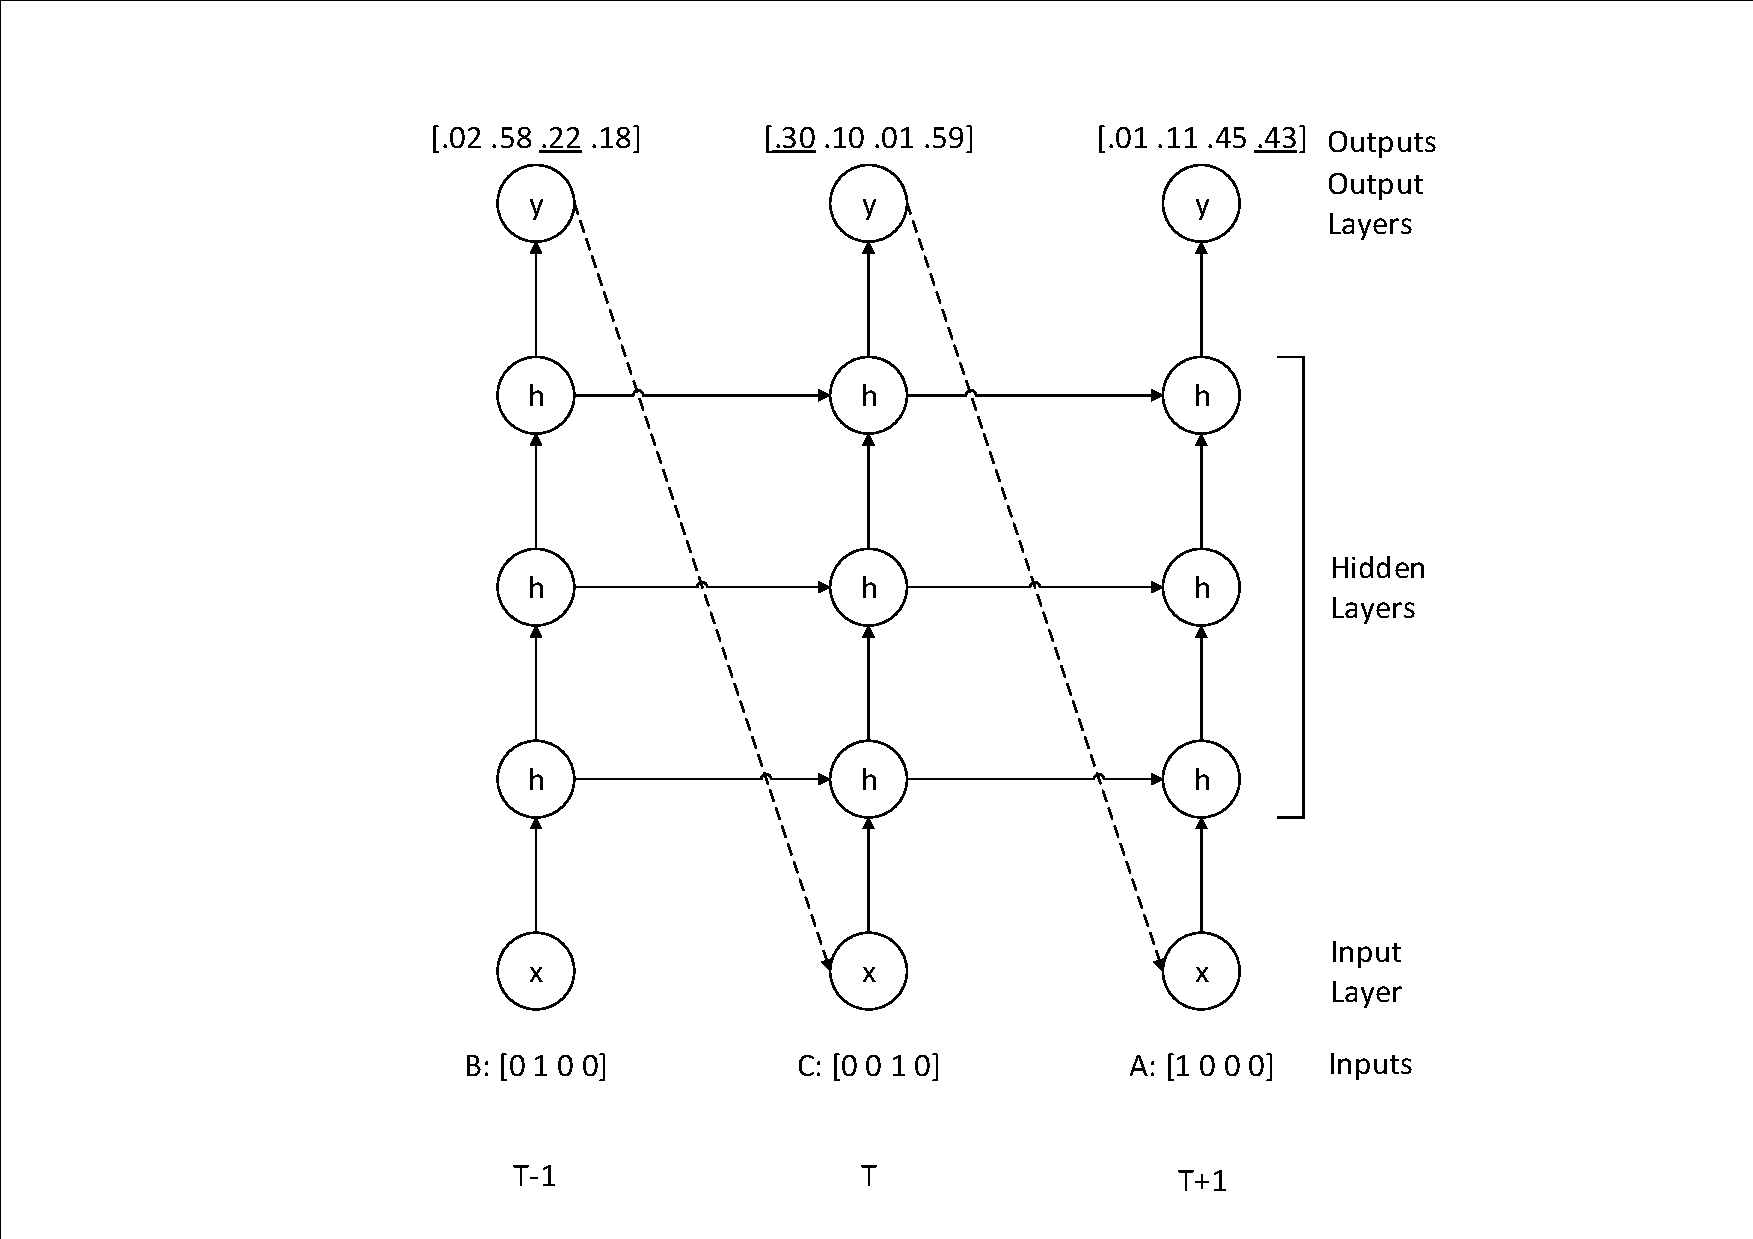
\includegraphics[width=\textwidth, trim = 4 4 4 4, clip, keepaspectratio]{images/char-rnn.pdf}
	\centering 
	\caption{Το μοντέλο \en{char-rnn} ανεπτυγμένο στο χρόνο.}
	\label{fig:char-rnn}
\end{figure}

\subsection{Μοντέλο \en{labeled-char-rnn}}

Το δεύτερο μοντέλο είναι επίσης ένα αναδραστικό νευρωνικό δίκτυο με 3 κρυμμένα επίπεδα στοιχείων \en{LSTM}. 
Εκτός από ακολουθίες χαρακτήρων, το μοντέλο αυτό δέχεται και πληροφορία για το είδος του χαρακτήρα. 
Αντίστοιχα οι έξοδοι του, εκτός από προβλέψεις για τον χαρακτήρα, περιέχουν και προβλέψεις για το είδος του χαρακτήρα. Με τον τρόπο αυτό θα εξετάσουμε κατά πόσο τα \en{RNNs} μπορούν να εκμεταλλευτούν \en{a priori} γνώσεις για τον κώδικα. Σημειώνεται πως η συνάρτηση επιδόσεων αυτού του μοντέλου είναι γραμμικός συνδυασμός των επιμέρους επιδόσεων πρόβλεψης χαρακτήρα και είδους χαρακτήρα.

Έστω το λεξιλόγιο \en{A, B, C, T}.
Έστω επίσης πως δίνουμε το είδος των χαρακτήρων αυτών στο σύστημα με βάση το αν είναι φωνήεντα ή σύμφωνα.
Για την εκπαιδευτική ακολουθία  <<\en{BCAT}>> δίνουμε την κατάλληλη είσοδο όπως στο σχήμα \ref{fig:l-char-rnn}.
Θέλουμε να μεγιστοποιηθούν και πάλι οι υπογραμμισμένες πιθανότητες. Για την παραγωγή του επόμενου χαρακτήρα και του είδους του, δειγματοληπτούμε από κάθε κατανομή εξόδου ξεχωριστά.

\begin{figure}[h]
	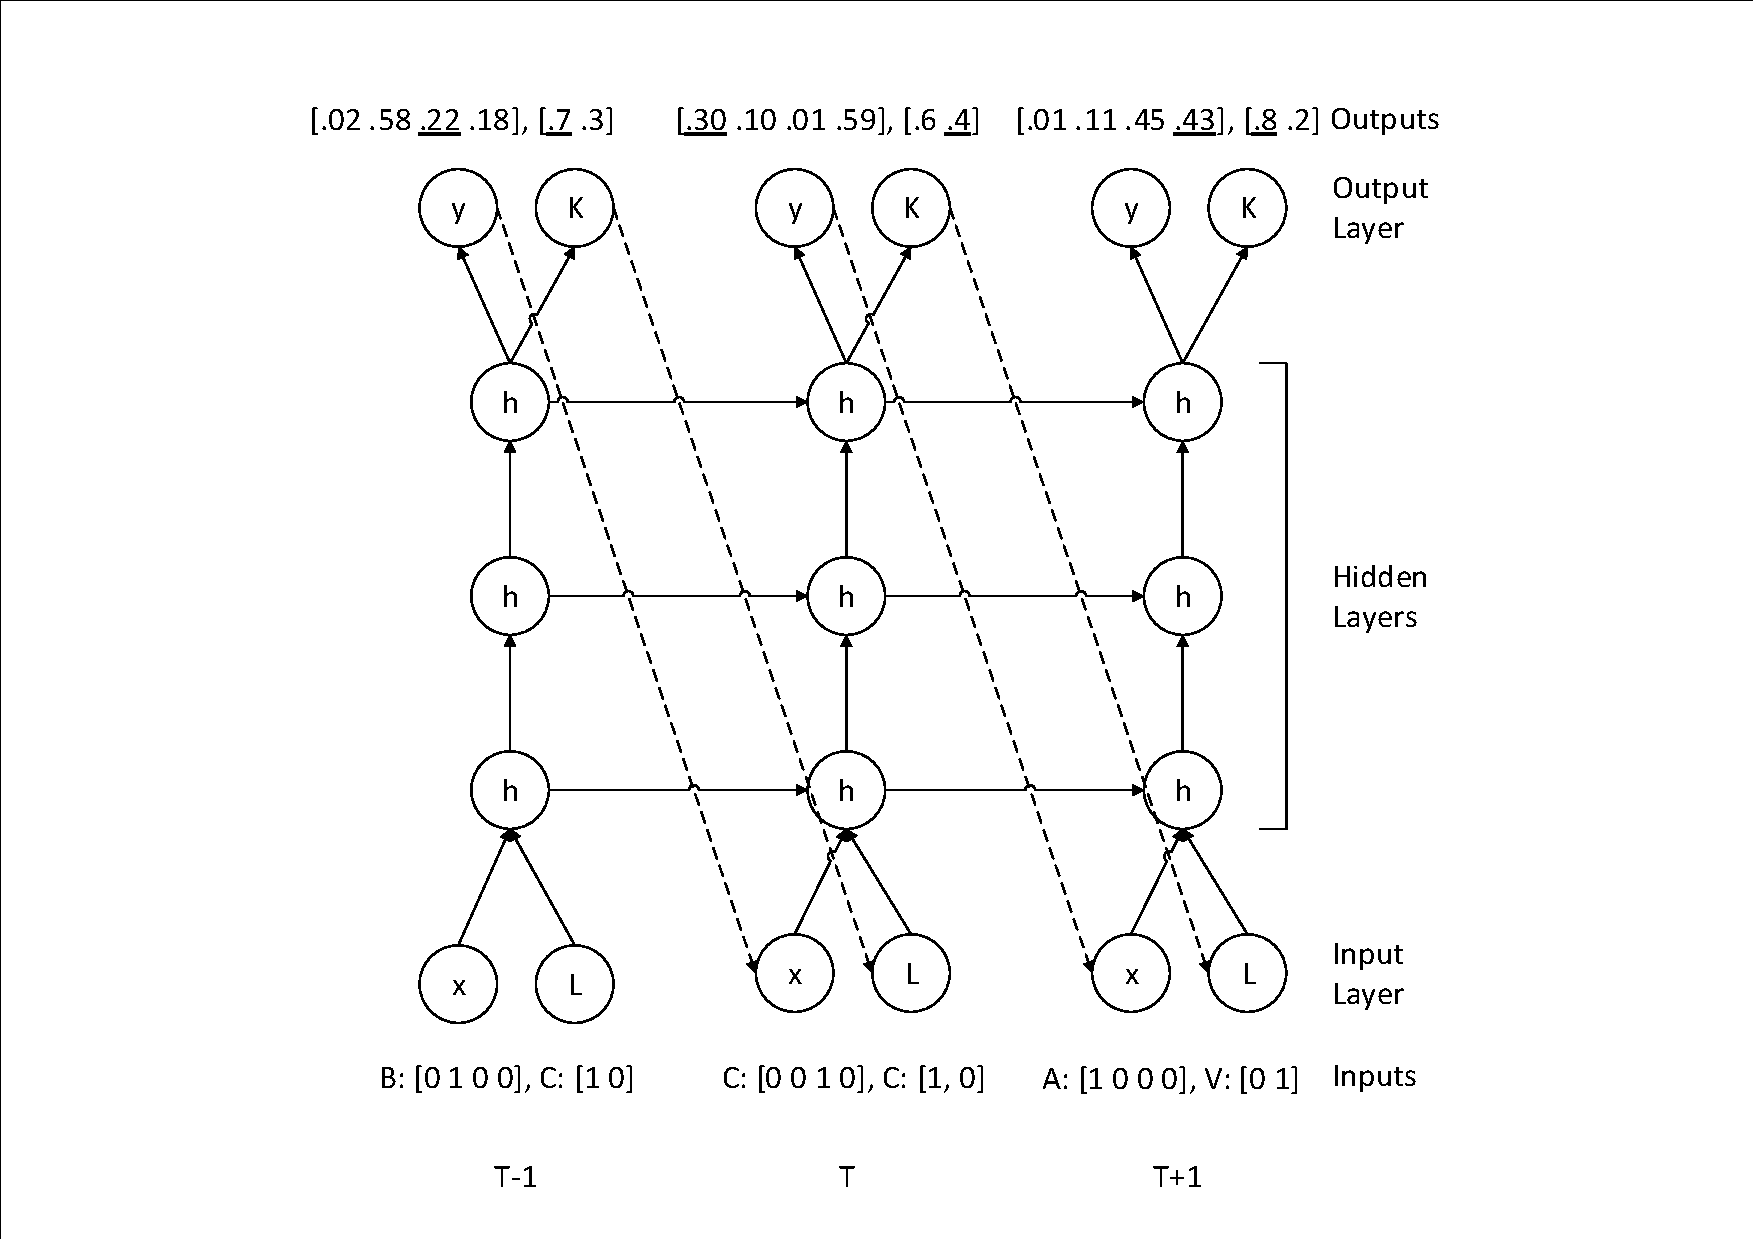
\includegraphics[width=\textwidth, trim = 4 4 4 4, clip, keepaspectratio]{images/l-char-rnn.pdf}
	\centering 
	\caption{Το μοντέλο \en{labeled-char-rnn} ανεπτυγμένο στο χρόνο.}
	\label{fig:l-char-rnn}
\end{figure}

\section{Προ-επεξεργασία}

Ο κορμός της διαδικασίας της προ-επεξεργασίας είναι ίδιος και για τα δύο σετ δεδομένων. 
Αρχικά αναζητούμε τα αρχεία με κατάληξη <<\en{.js}>> διασχίζοντας σειριακά όλους τους φακέλους των \en{projects}, εκτός από αυτούς που αφορούν \en{testing} και \en{localization}.
Ο έλεγχος για το τελευταίο γίνεται απλοϊκά, ελέγχουμε δηλαδή αν οι φάκελοι φέρουν τα συνήθη ονόματα που χρησιμοποιούνται για τέτοιου είδους φακέλους.
Ο μη ενδελεχής έλεγχος καταφέρνει να αφαιρέσει την πλειοψηφία των επαναλαμβανόμενων αρχείων αφήνοντας ένα μικρό ποσοστό να περάσει.
Αυτό έχει ως αποτέλεσμα να εμπλουτιστεί η εκπαίδευση του νευρωνικού, χωρίς όμως να μονοπωλείται το ενδιαφέρον από αρχεία που περιέχουν τετριμμένο κώδικα.
Στη συνέχεια, με τη βοήθεια ενός εργαλείου ανάλυσης της σύνταξης και γραμματικής προγραμματιστικών γλωσσών (ονόματι \en{\textit{linguist}}\footnote{\en{\url{https://github.com/github/linguist/}}}) προχωράμε στο περαιτέρω φιλτράρισμα αρχείων.
Συγκεκριμένα, εξαιρούμε αρχεία που έχουν την κατάληξη <<\en{.js}>> αλλά δεν είναι αρχεία κειμένου και αρχεία που είναι αυτόματα παραγώμενα και αποτελούν παραπροϊόν της διαδικασίας ανάπτυξης λογισμικού σε \en{JavaScript}.

\selectlanguage{english}
\lstinputlisting[language=JavaScript, caption={\tg{Αρχείο κώδικα πριν το }\en{minification}}]{code/beforemin.js}
\selectlanguage{greek}

\selectlanguage{english}
\lstinputlisting[language=JavaScript, caption={\tg{Αρχείο κώδικα μετά το }\en{minification}}]{code/aftermin.js}
\selectlanguage{greek}

Αφού επιλέξουμε τα αρχεία τα οποία θα αποτελούν το σετ δεδομένων μας προχωράμε στη διαδικασία της ελαχιστοποίησης του κώδικα (\en{minification, minimisation}).
Η ελαχιστοποίηση κώδικα, είναι η διαδικασία αφαίρεσης περιττών χαρακτήρων από των πηγαίο κώδικα, χωρίς να αλλάζει η λειτουργικότητά του. Τέτοιοι χαρακτήρες είναι τα κενά, τα σύμβολα αλλαγής παραγράφου, τα σχόλια και άλλα. Εδώ χρησιμοποιήθηκε το εργαλείο \en{\textit{jsmin}}\footnote{\en{\url{http://www.crockford.com/javascript/jsmin.html}}}. Οι κώδικες 4.1, 4.2 δείχνουν ένα αρχείο κώδικα πριν και μετά το \en{minification}.

Με την επιλογή αυτή προσπαθούμε να αφαιρέσουμε την περιττή πληροφορία απο τα δεδομένα μας, ώστε να είναι πιο εύκολο για το μοντέλο να αποτυπώσει τις σημαντικές σχέσεις ανάμεσα στους διάφορους χαρακτήρες.
Μετά το \en{minification} προσθέτουμε 2 ειδικούς χαρακτήρες για την αρχή και το τέλος κάθε αρχείου. Σημειώνεται πως θεωρούμε πως τα αρχεία ειναι \en{extended ASCII} κωδικοποιημένα και στην ουσία διαβάζουμε \en{bytes}.

Για την εκπαίδευση του μοντέλου \en{labeled-char-rnn} χρειάζεται να προετοιμάσουμε με ανάλογο τρόπο την πληροφορία για το είδος των χαρακτήρων. Για το σκοπό αυτό, χρησιμοποιούμε ένα άλλο εργαλείο ανάλυσης σύνταξης και γραμματικής προγραμματιστικών γλωσσών που φέρει το όνομα \en{\textit{pygments}}\footnote{\en{\url{http://pygments.org}}}.
Η επιλογή για τον διαχωρισμό των ειδών βασίζεται στα αυθαίρετα συντακτικά δέντρα (\en{abstract syntax trees}) της \en{JavaScript}, είναι όμως απλουστευμένη και δε χρησιμοποιεί δομές δέντρων, αλλά απλών διανυσμάτων.
Ο διαχωρισμός των χαρακτήρων γίνεται ανάμεσα στις ακόλουθες κλάσεις: \en{(\textbf{K}eyword, \textbf{N}umber, \textbf{R}egex, \textbf{S}tring, \textbf{O}perator, \textbf{P}unctuator, \textbf{I}dentifier).}

Οι χαρακτήρες και τα είδη τους αποθηκεύονται ως λίστες από αλφαριθμητικά στοιχεία ώστε να είναι διαθέσιμα ανά πάσα στιγμή στην εκπαιδευτική διαδικασία.
Προφανώς υπάρχει χρονική αντιστοιχία μεταξύ των αρχείων που περιέχουν της ακολουθίες χαρακτήρων με τα αρχεία που περιέχουν το είδος κάθε χαρακτήρα, όπως στα παραδείγματα του πίνακα \ref{label-example}.
Συνηθίζεται σε τέτοιου είδους προβλήματα να <<\tg{ανακατεύονται}>> οι ακολουθίες αλφαριθμητικών χαρακτήρων με σκοπό την .
Στα προβλήματα μάθησης έχουμε τη δυνατότητα να <<\tg{ανακατεύουμε}>> το σετ δεδομένων με σκοπό την γρηγορότερη/καλύτερη εκπαίδευση των μοντέλων.
Επειδή το ζητούμενο μας στη διπλωματική αυτή είναι η παραγωγή κώδικα, και η σειρά των ακολουθιών είναι άρρηκτα συνδεδεμένη με τη λειτουργικότητα και την ουσία των προγραμμάτων, δεν προχωράμε σε αυτή την επιλογή.  

\begin{table}[]
\centering
\caption{Παράδειγμα αντιστοιχίας χαρακτήρων με το είδος τους σε μια ακολουθία}
\label{label-example}
\begin{tabularx}{\textwidth}{|l|XXXXXXXXXXXXXXXXXXXXX|}
\hline
\en{String 1} & \en{v} & \en{a} & \en{r} &   & \en{a} & = & 1 & \en{;} & \en{f} & \en{u} & \en{n} & \en{c} & \en{t} & \en{i} & \en{o} & \en{n} &   & \en{f} & \en{(} & \en{A} & \en{)} \\ \hline
\en{Label 1}  & \en{K} & \en{K} & \en{K} & \en{P} & \en{I} & \en{O} & \en{N} & \en{P} & \en{K} & \en{K} & \en{K} & \en{K} & \en{K} & \en{K} & \en{K} & \en{K} & \en{P} & \en{I} & \en{P} & \en{I} & \en{P} \\ \hline
\hline
\en{String 2} & \{ & \en{r} & \en{e} & \en{t}  & \en{u} & \en{r} & \en{n} &  & < & \en{o} & \en{k} &  > & \en{;} & \} & \en{c} & = & \en{f} & \en{(} & \en{1} &\en{0} & \en{)} \\ \hline
\en{Label 2}  & \en{P} & \en{K} & \en{K} & \en{K} & \en{K} & \en{K} & \en{K} & \en{P} & \en{S} & \en{S} & \en{S} & \en{S} & \en{P} & \en{P} & \en{I} & \en{O} & \en{I} & \en{P} & \en{N} & \en{N} & \en{P} \\ \hline
\end{tabularx}
\end{table}

\section{Εκπαίδευση}


Η εκπαίδευση γίνεται στο \en{training set} του καθενός από τα δύο σετ δεδομένων. 
Οι χαρακτήρες δίνονται ως \en{\textit{one-hot}} διανύσματα, με μήκος όσο και οι διαφορετικοί χαρακτήρες του σετ δεδομένων.
Χρησιμοποιείται η τεχνική του \en{dropout}, ενώ ο αλγόριθμος που χρησιμοποιείται για την ελαχιστοποίηση του λάθους είναι ο \en{TBPTT}.
Η συνάρτηση λάθους είναι η \en{cross-entropy loss function}: $\sum_x p(x) \log{q(x)}$, όπου $p(x)$ είναι η πραγματική κατανομή των χαρακτήρων και $q(x)$ η προβλεπόμενη κατανομή χαρακτήρων του μοντέλου.
Η συνάρτηση αυτή χρησιμοποιείται στην πλειοψηφία της σύγχρονης βιβλιογραφίας και εμπειρικά έχει καλά αποτελέσματα στην εκπαίδευση των αναδραστικών νευρωνικών δικτύων.
Εξίσου ευρεία χρήση συναντά και η συνάρτηση \en{\textit{rmsprop}} που χρησιμοποιούμε για τη βελτιστοποίηση του \en{gradient descent}.

Η εκπαίδευση του αναδραστικού νευρωνικού δικτύου γίνεται, πιο περιγραφικά ως εξής: δείχνουμε στο νευρωνικό δίκτυο ακολουθίες σταθερού μήκους, το οποίο προαποφασίζεται της εκπαίδευσης.
Ως αληθείς απαντήσεις δίνουμε ένα διάνυσμα ίσου μήκους με το προηγούμενο που περιέχει τους χαρακτήρες της επόμενης χρονικής στιγμής (κύλιση του διανύσματος κατά μία θέση).
Στην περίπτωση του μοντέλου  \en{labeled-char-rnn} με όμοιο τρόπο δίνονται και οι πληροφορίες σχετικά με το είδος των χαρακτήρων, μαζί με τους αντίστοιχους χαρακτήρες.
Με σκοπό την παραλληλοποίηση του προγράμματος, δίνουμε πολλά τέτοια παραδείγματα ταυτόχρονα.

Συνολικά εκπαιδεύουμε 4 διαφορετικά μοντέλα. Για κάθε \en{dataset} το αντίστοιχο \en{char-rnn} και \en{labeled-char-rnn} μοντέλο.
Για την εκπαίδευση των μοντέλων, πρέπει να αποφασιστεί ένα σύνολο παραμέτρων, που φέρουν σημαντική αξία για τις τελικές επιδόσεις του μοντέλου και την διάρκεια της εκπαίδευσης. Αυτές είναι:

\begin{itemize} 
\item Μήκος ακολουθίας \en{(Sequence length)}: Ο αριθμός χαρακτήρων που περιέχει μία ακολουθία.
\item Μέγεθος παρτίδας \en{(Batch size)}: Ο αριθμός των εκπαιδευτικών ακολουθιών που δίνονται παράλληλα στο μοντέλο.
\item Μέγεθους κρυμμένων επιπέδων \en{(Hidden state size)}: Ο αριθμός των στοιχείων \en{LSTM} που απαρτίζουν κάθε κρυφό επίπεδο.
\item Πιθανότητα \en{dropout}: Η πιθανότητα να κρατηθεί ένα στοιχείο στη διάρκεια τη εκπαίδευσης.
\item Αριθμός εποχών \en{(Epoch number)}: Ο αριθμός <<περασμάτων>> του τεστ δεδομένων.
\item Ρυθμός εκμάθησης \en{(Learning rate)}: Πόσο γρήγορα μαθαίνει το σύστημα από τα λάθη του.

\end{itemize}

Για την στρατηγική επιλογής και την ακριβή τιμή των υπερ-παραμέτρων θα μιλήσουμε στο Κεφάλαιο 5.

\section{Παραγωγή}

Το μοντέλο που επιλέγουμε για καθένα από τα πειράματα αποφασίζεται σύμφωνα με τις επιδόσεις του στην μετρική λάθους της εκπαίδευσης.
Για να είναι ευκολότερα ερμηνεύσιμα τα αποτελέσματα της εκπαίδευσης, θα χρησιμοποιούμε και την μετρική της <<\tg{ευστοχίας}>>.
Η ευστοχία είναι το ποσοστό επιτυχημένων προβλέψεων επόμενου χαρακτήρα σε μία παρτίδα.

Η διαδικασία παραγωγής κώδικα που περιγράψαμε γενικεύεται και για τα μοντέλα που περιέχουν πληροφορία για το είδος των χαρακτήρων.
Μπορούμε δηλαδή να δειγματοληπτούμε από την προβλεπόμενη κατανομή για τα είδη των χαρακτήρων και να χρησιμοποιούμε το αποτέλεσμα ως επόμενη είσοδο.
Μπορούμε επίσης να οδηγήσουμε έμμεσα το σύστημα, αρχικοποιώντας το με κώδικα της επιλογής μας. Αυτό αλλάζει την εσωτερική κατάσταση του μοντέλου και το <<προϊδεάζει>> για το τι κώδικας μπορεί να ακολουθεί. 
Επιπρόσθετα, κατά τη διάρκεια της δειγματοληψίας έχουμε τη δυνατότητα να επηρεάσουμε την κατανομή που προτείνει το μοντέλο.
Αυτό ελέγχει το μοντέλο ως προς τη <<σιγουριά>> του για τις προβλέψεις του και έχει τη δυνατότητα να κάνει τον παραγώμενο κώδικα, είτε πιο ντετερμινιστικό, είτε πιο ποικίλο.
Σημαντική ιδιότητα αυτής της προσθήκης είναι πως δίνει στο μοντέλο τη δυνατότητα να ξεφύγει από φαύλους κύκλους ντετερμινιστικών λαθών χάρη στην επιπλέον τυχαιότητα που εισάγεται.
Η συνάρτηση ονομάζεται \en{\textit{Softmax Temperature}} και είναι: 

\begin{ceqn}
\begin{align}
P = \frac{e^{y/T}}{\sum_{k = 1}^{n} e^{y_k/T}}
\end{align}
\end{ceqn}

Όπου $P$ είναι η νέα κατανομή, $y$ είναι η εξαγόμενη του νευρωνικού δικτύου πιθανοτική κατανομή και $n$ ο αριθμός των διαφορετικών στοιχείων προς πρόβλεψη. $T$ είναι η τιμή της θερμοκρασίας που επηρεάζει την  κατανομή.
Για τιμές μεγαλύτερες του 1, ο κώδικας γίνεται πιο ποικίλος, αλλά με περισσότερα λάθη.
Τιμές μικρότερες του 1 έχουν ως αποτέλεσμα το σύστημα να είναι πιο σίγουρο για τις προβλέψεις του.




\chapter{Πειράματα και Αποτελέσματα}

Στο κεφάλαιο αυτό θα αναλύσουμε τα πειράματα που έγιναν για την εκπαίδευση του μοντέλου παραγωγής κώδικα και θα εξετάσουμε την ποιότητα του παραγώμενου κώδικα.
Θα εξετάσουμε ξεχωριστά κάθε σετ δεδομένων και θα συγκρίνουμε τις επιλογές και τις επιδόσεις των 2 προσεγγίσεων σε καθ' ένα απο αυτά.
Τέλος θα ελέγξουμε τις επιδόσεις του μοντέλου σε ένα υπο-προΪόν της λειτουργίας του, στην αυτόματη συμπλήρωση κώδικα.


\section{Πειράματα εκπαίδευσης}

Ένα πολύ σημαντικό κομμάτι της εκπαίδευσης ενός τέτοιου συστήματος είναι η κατάλληλη επιλογή των υπερπαραμέτρων.
Αποδεικνύεται πως η αποδοτικότερη μέθοδος για την επιλογή τους είναι η τυχαία μέθοδος \cite{Bersgstra2012}.
Η υπολογιστική πολυπλοκότητα που εισάγουν τα αναδραστικά νευρωνικά δίκτυα και οι περιορισμένοι υπολογιστικοί πόροι που έχουμε στη διάθεση μας κάνουν αυτή την επιλογή αδύνατη.
Αντ' αυτού επιλέγουμε εμπειρικά τις υπερπαραμέτρους (με δοκιμές) και με οδηγό της επιλογές στη σύγχρονη σχετική βιβλιογραφία.

\subsection{\en{Top 100 Github Javascript Projects} Πειράματα}

To σετ δεδομένων αυτό αποτελείται από τα 100 πιο δημοφιλή \en{projects} σε γλώσσα \en{javascript} στον ιστότοπο αποθετηρίων λογισμικόυ \en{github}.
Μετά τo prepocessing παίρνουμε ακολουθίες συνολικού μήκους περίπου 79 εκατομμυρίων χαρακτήρων.
Υπάρχουν 212 διαφορετικοί χαρακτήρες, συμπεριλαμβανομένων των ειδικών χαρακτήρων αρχής και τέλους αρχείων.
Χρησιμοποιούμε το 95\% των δεδομένων για την εκπαίδευση του συστήματος και το υπόλοιπο 5\% για την επικύρωση της μάθησης.
Η έλλειψη ξεχωριστού τεστ σετ μπορεί να σημαίνει οτι τα αποτελέσματα μας κάνουν overfit στα δεδομένα επικύρωσης, αλλά αυτό είναι δευτερευούσης σημασίας αφού στόχος μας είναι να παράξουμε κώδικα και δεν υπάρχει αντικειμενική μαθησιακή μετρική για τον σκοπό αυτό.

Η στρατηγική επιλογής των παραμέτρων έχει ως εξής: Για να είναι οι δύο προσεγγίσεις συγκρίσιμες κρατάμε ίδιο το μέγεθος των κρυφών επιπέδων.
Από αυτή την επιλογή εξαρτάται κυρίως ο αριθμός συνολικών παραμέτρων προς εκπαίδευση.
Για το πρώτο σετ δεδομένων αποφασίζουμε τον αριθμό αυτό σε 1024, αριθμός αρκετά μεγάλος ωστε να ειναι αντιμετωπίσιμο από το σύστημα το ογκώδες σετ δεδομένων.

Η επόμενη υπερ-παράμετρος που πρέπει να αποφασιστεί είναι το μήκος της εκπαιδευτικής ακολουθίας, η μεταβλητή $k_2$ του αλγορίθμου \en{TBPTT}.
Η υπερ-παράμετρος αυτή έχει μεγάλη σχέση τόσο με την ποιότητα του παραγώμενου κώδικα, αφού ελέγχει πόσους από τους προηγούμενους χαρακτήρες <<βλέπει>> το σύστημα, αλλά και με τον χρόνο εκτέλεσης μιας εποχής, αφού μεγαλύτερες ακολουθίες εισάγουν υπολογιστική πολυπλοκότητα.
Το μέγεθος των εκπαιδευτικων ακολυθιών αποφασίζεται στους 100 χαρακτήρες και για τα δύο μοντέλα.

Ο ρυθμός εκμάθησης είναι άμεσα συνδεδεμένος με το μέγεθος παρτίδας.
Όσο περισσότερα παραδείγματα βλέπει ταυτόχρονα το σύστημα τόσο πιο σίγουρο θα πρέπει να είναι για τα συμπεράσματα του.
Εξαγωγή δυνατών συμπερασμάτων απο λιγοστά παραδείγματα πρέπει να αποφεύγεται.
Επιπρόσθετα υπάρχει και ένας φυσικός περιορισμός στο πόσα παραδείγματα μπορούν να δείχνονται ταυτόχρονα, η μνήμη της επεξεργαστικής μας μονάδας.
Τελικώς δείχνουμε 200 ακολουθίες σε κάθε βήμα εκμάθσης και θέτουμε τον ρυθμό εκμάθησης στην τιμή 0.002, ωστέ να γεμίζουμε όσο καλύτερα γίνεται την μνήμη του υπολογιστικού συστήματος αλλά να συνεχίσουμε να μαθαίνουμε αποτελεσματικά.
Σημειώνεται πως η προτεινόμενη τιμή για τον ρυθμό εκμάθησης της \en{rmsprop} είναι το 0.001.

Τέλος, επειδή το σετ δεδομένων αυτό είναι αρκετά ογκώδες και περίπλοκο, είναι δύσκολο το μοντέλο μας να κάνει overfit. Έτσι, δε χρείαζεται η πιθανότητα dropout να είναι εξαιρετικά μεγάλη.
Επιλέγουμε την υπερπαράμετρο αυτή στο 20\%, ενώ η γενική προτεινόμενη τιμή είναι 40\% με 50\%.
Ο αριθμός των εποχών αποφασίζεται έτσι ώστε κανένα από τα 2 μοντέλα να μην βελτιώνει τις επιδόσεις του στο σετ δεδομένων επιβεβαίωσης.
Ο αριθμός αυτός προκύπτει στις 60 εποχές.
Στον πίνακα \ref{hyper1} παρουσιάζονται συνοπτικά οι παραπάνω αποφάσεις.

\begin{table}[]
\centering
\begin{tabularx}{\textwidth}{|X|X|X|}
\hline
                    & \en{char-rnn} & \en{labeled-char-rnn} \\
\hline
\en{\#} Παραμέτρων       & 23Μ             & 23Μ                     \\
\hline
\en{\#} Χαρακτήρων       & 212             & 212, 8                  \\
\hline
\en{\#} Εποχών       & 40             & 60                  \\
\hline
Μέγεθος \en{LSTM}  & 1024            & 1024                    \\
\hline
Μήκος Ακολουθίας    & 100             & 100                     \\
\hline
Ρυθμός Εκμάθησης    & 0.002           & 0.002                   \\
\hline
\% \en{Dropout}     & 20              & 20                      \\
\hline
Μέγεθος Παρτίδας    & 200             & 200                     \\
\hline
\end{tabularx}
\caption{Υπερπαράμετοι για τα \en{top 100 Github js projects}}
\label{hyper1}
\end{table}

Η εκπαίδευση έγινε σε μία κάρτα γραφικών \en{Nvidia Gtx 960} με 4 \en{gb RAM}.
Η εκπαίδευση διαρκεί 6 περίπου ημέρες για το πρώτο μοντέλο και 7 περίπου για το δεύτερο.
Όπως αναφέραμε, η παρακολούθηση των επιδόσεων και η επιλογή των σετ βαρών για την παραγωγή κώδικα γίνεται σύμφωνα με την μετρική \en{Average cross entropy per minibatch}.
Σημειώνεται πως η σύγκριση των μοντέλων στην μετρική αυτή γίνεται μόνο στο κομμάτι που αφορά την πρόβλεψη χαρακτήρων.
Στην εικόνα \ref{training1} φαίνεται η εξέλιξη της εκπαίδευσης των 2 μοντέλων στην περίοδο 40 και 60 εποχών στο σετ εκπαίδευσης και το σετ επαλήθευσης. 
%TODO Διάγραμμα training me σχόλια περι overfittinh και τετοια και επιλογής μοντέλο και ξαναγραψιμο της μετρικής που χρησιμοποιείται 1 + 0.2. Σχολιασμός των accuracy
Ως μοντέλα παραγωγής, επιλέγουμε αυτά με τα βάρη τις 38ης εποχής για το μοντέλο \en{char-rnn} και της 53 εποχής για το μοντέλο \en{labeled-char-rnn}, αφού παρουσιάζουν την ελάχιστη τιμή της μετρικής μας.
Οι επιδόσεις των μοντέλων αυτών αντιστοιχόυν σε 85.6\% και 87.2\% ποσοστιαία επιτυχία στην πρόβλεψη του επόμενου χαρακτήρα.
Η επιτυχία πρόβλεψης του είδους του χαρακτήρα στο σετ επαλήθευσης βρίσκεται πάνω από το 97\%.
Τα αποτελέσματα της εκπαιδευτικής διαδικασίας είναι σε πρώτη όψη ικανοποιητικά. Οι καμπύλες εκπαίδευσης και επαλήθευσης μένουν σε κοντινά επίπεδα και για τα δύο μοντέλα, γεγονός που μαρτυρά καλή γενίκευση τών χαρακτηριστικών που μαθαίνονται. Η εκμάθηση, ιδιαίτερα, της ανάθεσης είδους στον επόμενο χαρακτήρα κυμαίνεται σε πολύ υψηλά επίπεδα. 

\begin{figure}[h]
	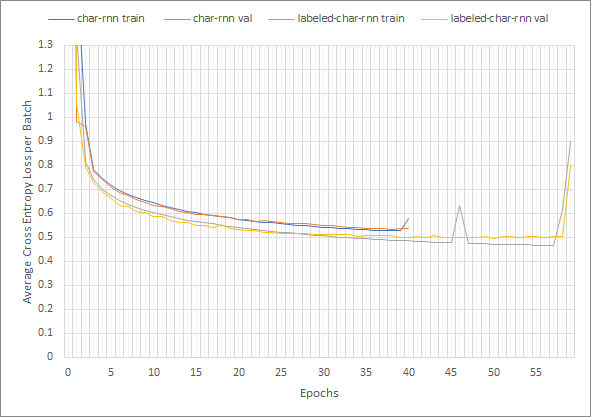
\includegraphics[trim = 2 2 2 2, clip, keepaspectratio]{images/training1.png}
	\centering
	\caption{Καμπύλες εκμάθησης για τα \en{top 100 github js projects}}
	\label{training1}
\end{figure}

\subsection{\en{Top 200 npm Projects} Πειράματα}

Το δεύτερο σετ δεδομένων αποτελείται από τις 200 πιο δημοφιλείς βιβλιοθήκες \en{javascript} του ιστοχώρου www.npmjs.com.
Οι ακολουθίες μετά την προ-επεξεργασία αριθμούν περίπου 49 εκατομμύρια χαρακτήρες με 210 διαφορετικούς χαρακτήρες. 
Σε αυτό το πείραμα χωρίζουμε το 90\% των ακολουθιών στο σετ εκπαίδευσης και το 10\% στο σετ επαλήθευσης, επειδή έχουμε λιγότερα δεδομένα και θέλουμε να αποφύγουμε μεγάλη διακύμανση στο σετ επαλήθευσης.

Οι αποφάσεις των υπερπαραμέτρων βασίζονται στις παρατηρήσεις μας από τα προηγούμενα πειράματα. Έτσι, κρατάμε ίδιο το μέγεθος παρτίδας, τον ρυθμό εκμάθησης και το μήκος ακολουθίας.
Το σετ εκπαίδευσης έχει μικρότερο μέγεθος από το προηγούμενο πείραμα και από τις πρώτες δοκιμές παρατηρούμε σημαντικό \en{overfitting}.
Προς την κατεύθυνση καλύτερης γενίκευσης των συμπερασμάτων του συστήματος, αρχικά μικραίνουμε το δίκτυο θέτοντας το μέγεθος \en{LSTM} se 700, κίνηση η οποία μειώνει σημαντικά τις εκπαιδεύσιμες παραμέτρους του συστήματος.
Έπειτα αυξάνουμε την πιθανότητα \en{dropout} σε 30\% και 40\% που αποτέλεσμα έχει την αργήτερη εκπαίδευση του αναδραστικού νευρωνικού δικτύου.
Για να αποζημιώσουμε την τελευταία μας επιλογή αυξάνουμε τις εκπαιδευτικές εποχές του μοντέλου σε 60 και 80 αντίστοιχα.
Οι εκπαιδευτικές επιλογές συνοψίζονται στον πίνακα \ref{hyper2}.

\begin{table}[]
\centering
\begin{tabularx}{\textwidth}{|X|X|X|}%TODO Check these values
\hline
                    & \en{char-rnn} & \en{labeled-char-rnn} \\
\hline
\en{\#} Παραμέτρων       & 10M             & 10M                     \\
\hline
\en{\#} Χαρακτήρων       & 210             & 210, 8                  \\
\hline
\en{\#} Εποχών       & 60             & 80                  \\
\hline
Μέγεθος \en{LSTM}  & 700            & 700                    \\
\hline
Μήκος Ακολουθίας    & 100             & 100                     \\
\hline
Ρυθμός Εκμάθησης    & 0.002           & 0.002                   \\
\hline
\% \en{Dropout}     & 30              & 40                      \\
\hline
Μέγεθος Παρτίδας    & 200             & 200                     \\
\hline
\end{tabularx}
\caption{Υπερπαράμετοι για τα \en{top 200 npm js libaries}}
\label{hyper2}
\end{table}

Η διαδικασία που ακολουθείται είναι η ίδια με του προηγούμενου πειράματος, δηλαδή εκπαιδεύουμε το σύστημα σε μία κάρτα γραφικών \en{Nvidia Gtx 960} με 4 \en{gb RAM} και επιλέγουμε το μοντέλο με τις καλύτερες επιδόσεις στη μετρική πρόβλεψης χαρακτήρων.
Η εκπαίδευση του \en{char-rnn} διαρκεί 3 ημήρες ενώ του \en{labeled-char-rnn} διαρκεί περίπου 4. Η εξέλιξη της εκπαίδευσης φαίνεται στην εικόνα \ref{training2}.

\begin{figure}[h]
	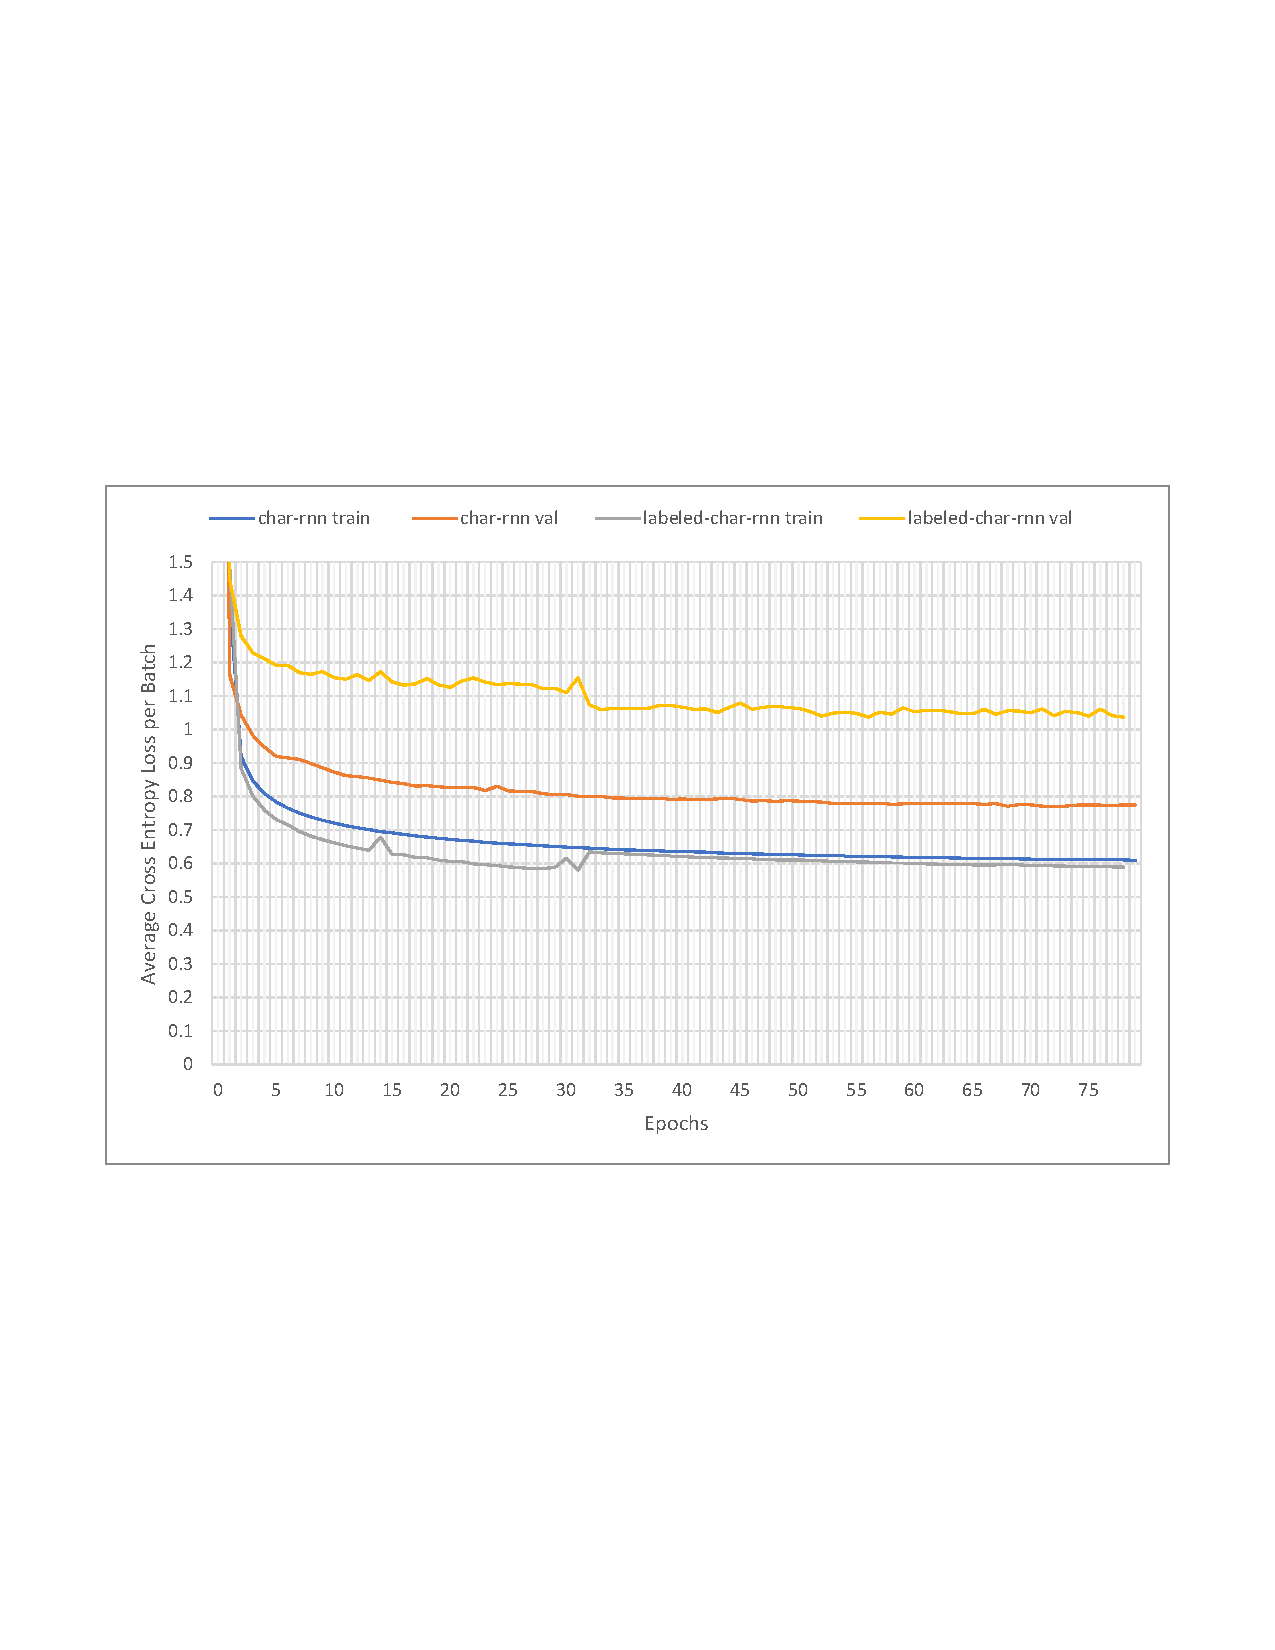
\includegraphics[width=\textwidth, trim = 25 220 25 220, clip, keepaspectratio]{images/training2.pdf}
	\centering
	\caption{Καμπύλες εκμάθησης για τα \en{top 100 github js projects}}
	\label{training1}
\end{figure}


Το επιλεγόμενο μοντέλο για το \en{char-rnn} είναι αυτό της 72ης εποχής με ποσοστό επιτυχίας πρόβλεψης 78\%. Για το μοντέλο \en{labeled-char-rnn} το επιλεγόμενο μοντέλο είναι αυτό της 78ης εποχής με ποσοστό επιτυχίας 72.3\% την πρόβλεψη χαρακτήρων και 94.7. Είναι εμφανές από το διάγραμμα οτι τα μοντέλα μας δυσκολεύονται περισσότερο να γενικεύσουν τα συμπεράσματα που εξάγουν από αυτό το σετ δεδομένων. Η ικανότητα πρόβλεψης του είδους του επόμενου χαρακτήρα παραμένει σε σχετικά υψηλά επίπεδα αλλα η προσθήκη της δεν βελτιώνει τις επιδόσεις στο σετ επιβεβαιωσης. Θα εξετάσουμε αναλυτικότερα τα αποτελέσματα αυτά στο υποκεφάλαιο των αποτελεσμάτων και στο κεφάλαιο των συμπερασμάτων.
%TODO Maybe add a side experiment subsevtion.

\section{Αποτελέσματα}

Χρησιμοποιούμε τα μοντελα που εκπαιδεύτηκαν παραπάνω για να παράξουμε 100 αρχεία κώδικα για κάθε προσέγγιση και κάθε ομάδα μοντέλων.
Επιλέγουμε ένα \en{javascript} project με το οποίο αρχικοποιούμε κάθε ομάδα μοντέλων. 
Αρχικά θα εξετάσουμε την ποιότητα του κώδικα εποπτικά και έπειτα θα χρησιμοποήσουμε το εργαλείο \en{jshint} για να κάνουμε στατική ανάλυση του κώδικα.

\subsection{\en{Top 100 Github Javascript Projects} Παραγώμενος κώδικας}

Η αρχικοποίηση του μοντέλου γίνεται με σκοπό την οδήγηση του.
Επιλέγουμε ένα project που δεν έχει εμφανιστεί στη διάρκεια της εκπαίδευσης και της επαλήθευσης.
Συγκεκριμένα επιλέγουμε το \en{hyper terminal} που είναι το πιο δημοφιλές \en{javascript project} στο \en{github} το πρώτο εξάμηνο του 2017.
Ο κώδικας 5.1 είναι ένα αρχείο από το \en{project} αυτό.

\selectlanguage{english}
\lstinputlisting[language=JavaScript, caption={\tg{Δείγμα κώδικα απο το }\en{hyper terminal}}]{code/hyper.js}
\selectlanguage{greek}

Όι κώδικες 5.2, 5.3 είναι δημιουργήματα των μοντέλων \en{char-rnn} και \en{labeled-char-rnn} αντίστοιχα. Τα αρχεία αυτά επιλέχτηκαν χάρη στο μικρό μέγεθός τους και την συντακτική ορθότητα.

\selectlanguage{english}
\lstinputlisting[language=JavaScript, caption={\tg{Δείγμα κώδικα απο το }\en{char-rnn}}]{code/charrnnGithub.js}
\selectlanguage{greek}

Ήδη εποπτικά παρατηρούμε τη δυνατότητα και των δύο μοντέλων να αναπαράγουν συντακτικές δομές, όπως οι παρενθέσεις και οι αγκύλες, αλλα και λογικές, όπως οι συναρτήσεις και οι δομές πολλαπλών επιλογών.
Φαινομενικά αυτό είναι ένα συνηθισμένο αρχείο \en{javascript}.
Με μία δεύτερη, αναλυτικότερη ματιά παρατηρούμε σημαντικά λάθη στη χρήση μη ορισμένων μεταβλητών, την ύπαρξη γραμματικών λαθών και ενέργειες χωρίς αποτέλεσμα. 
Είναι εύκολο να συμπεράνει κανείς, ίσως και χωρίς να είναι γνώστης της γλώσσας, πως τα προγράμματα αυτά δεν θα καταφέρουν να μεταφραστούν. 
Για την καλύτερη εκτίμηση των αποτελεσμάτων των νευρωνικών δικτύων, και για τη σύγκριση των δύο  θα ακολουθήσουμε μια πιο ποσοτική προσέγγιση. 
Με τη χρήση του εργαλείόυ ανάλυσης κώδικα \en{jshint} θα εξετάσουμε τον αριθμό των συντακτικών λαθών που εντοπίζονται και μέχρι πιο σημείο καταφέρνουν να αναγνωστούν πριν βρεθεί ένα ανεπανόρθωτο συντακτικό λάθος.
Σημειώνεται πως τα μοντέλα αποφασίζουν αυτόνομα το μήκος του κώδικα, με τη χρήση των ειδικών χαρακτήρων, αλλά τίθεται ένα άνω όριο 15000 χαρακτήρων στο οποίο θεωρούμε οτι το αρχείο ξεφεύγει διαχειρισμότητας λόγω μεγέθους.
% Σημειώνεται πως τα μοντέλα αποφασίζουν αυτόνομα το μήκος του κώδικα, με τη χρήση των ειδικών χαρακτήρων, αλλά τίθεται ένα άνω όριο 15000 χαρακτήρων στο οποίο θεωρούμε οτι το αρχείο ξεφεύγει διαχειρισμότητας λόγω μεγέθους.
Στις εικόνες ρεφ ρεφ φαίνονται τα αποτελέσματα της παραπάνω ανάλυσης και το μήκος των παραγώμενων αρχείων.
% Στις εικόνες ref ref φαίνονται τα αποτελέσματα της παραπάνω ανάλυσης και το μήκος των παραγώμενων αρχείων.

\selectlanguage{english}
\lstinputlisting[language=JavaScript, caption={\tg{Δείγμα κώδικα απο το }\en{char-sssrnn}}]{code/labeledcharrnnGithub.js}
\selectlanguage{greek}


% References imported from `references.bib'. 
%IMPORTANT: Manually modify `main.bbl' by adding \selectlanguage{english} (TOP) and \selectlanguage{english} (BOTTOM) in order to correctly display Latin and Greek characters in the final text.
%TODO create .tex file for bibliography, in order to have greek heading in the bibliography page
\bibliography{references}


\appendix
%\include{proofs}

\newcommand{\gloss}[2]{#1 \> \en{#2}\\ }

\chapter{����������� ����� ����}

\begin{tabbing}
%ta 'a' rythmizoun to platos ton dyo stilon
  aaaaaaaaaaaaaaaaaaaaaaaaaaaaaaaaaaa \= aaaa\kill
  \Large\textbf{���������} \> \Large\textbf{�������� ����} \\
  \gloss{�������}{sibling}
  \gloss{��������������}{idempotency}
  %\gloss{������������}{identifier}
  \gloss{�������� �����������}{information retrieval}
  \gloss{������������������}{commutativity}
  \gloss{��������}{descedant}
  \gloss{����������}{absorption}
  \gloss{���� ���������}{database}
  \gloss{��������}{attribute}
  \gloss{������������}{interface}
  \gloss{�������}{difference}
  \gloss{��������� ���������}{portal catalog}
  \gloss{�������� ����}{lattice}
  \gloss{������� �����������}{structural queries}
  \gloss{������� �������}{structural relationships}
  \gloss{������ �����}{schema}
  \gloss{����������}{validity}
  \gloss{�����}{union}
\end{tabbing}


\backmatter
\printindex

\end{document}